\documentclass[10pt,a4paper]{report}
\usepackage{hyperref}	%Muss ganz am Anfang geladen werden: https://tex.stackexchange.com/a/126454
\usepackage{url}
\usepackage[utf8]{inputenc}
\usepackage{amsmath}
\usepackage{amsfonts}
\usepackage{amssymb}
\usepackage{listings}
\usepackage{struktex}
\usepackage{gensymb}

\usepackage[ngerman]{babel}

\usepackage{tikz,pgfplots}
%%%%<
%\usepackage{verbatim}
%\usepackage[active,tightpage]{preview}
%\PreviewEnvironment{tikzpicture}
%\setlength\PreviewBorder{5pt}%
%%%%>

\usetikzlibrary{arrows,%
                shapes,positioning}

\begin{document}

\chapter{Aufgabenstellung}

Im Rahmen des Praktikums sind aus Geoterraindaten mögliche Notlandebahnen für Notfallsituationen im Luftverkehr zu ermitteln. Im Falle eines vollständigen Turbinenausfalls kann es z.B. vorkommen, dass der nächstgelegene Flughafen auf Grund aktueller Flughöhe und Windrichtung nicht mehr erreicht werden kann.

Innerhalb der zur Verfügung gestellten Geländedaten, die im GeoTiff Format vorliegen, soll ein Algorithmus entwickelt werden, der plane Flächen darin ermittelt, die sich zum Landen eines Flugzeugs eigenen.

Die Eignung einer Landebahn ergibt sich aus Parametern wie Länge, Breite, Winkel, Steigung, Holprigkeit und Querneigung der Bahn.
Diese werden der Software zur Ermittlung mitgegeben und die Software findet dann Landebahnen, die diesen Kriterien entsprechen.
Insbesondere Breite und Länge der Landebahn müssen konfigurierbar sein, da ein Ultraleichtflugzeug und eine Verkehrsmaschine wie ein Airbus A380 oder eine Boeing 767 völlig unterschiedliche Vorgaben benötigen.

Weiterhin ist der Winkel der Bahn im Zusammenspiel mit den aktuellen vorherrschenden Windverhältnissen von großer Bedeutung. 
Ein weiterer Fokus dieses Praktikums liegt in der Anwendung von Parallelverarbeitung.

Im speziellen soll eine Parallelisierung mit p\_threads durchgeführt werden, also eine klassische Shared Memory Architektur.
Es soll untersucht werden, wie sich der Speed-up mit zunehmender Anzahl an Threads verhält und mit der seriellen Abarbeitung verglichen werden.

Die gefundenen Landebahnen sind dann in einem UI zu visualisieren.

Die Software soll dem Piloten eine Entscheidungshilfe sein und mögliche Optionen anbieten. Insbesondere die Kombination von Notfall und der teilweise stark eingeschränkten Sicht im Cockpit soll durch eine technische Unterstützung die Entscheidungsfindung erleichtern.
Die Landung selbst soll nach wie vor von einem Menschen durchgeführt werden. Fragestellungen wie Fahrwerk ein- oder ausfahren bleiben hier außen vor.     

\chapter{Architektur}

Zur Lösung der Aufgabenstellung muss zunächst eine Systemarchitektur festgelegt werden.

\section{Überblick}
Zum Einlesen der Rohdaten, Steuern der Applikation und zum Auffinden, Persisitieren und Anzeigen der potentiellen Notlandefelder sind vielfältige Schritte notwendig. Diese haben jeweils ihre eigenen spezifischen Herausforderungen und sind bei näherer Betrachtung sogar relativ unabhängig voneinander lösbar.

Daraus ergibt sich die Möglichkeit das System aus relativ lose gekoppelten Komponenten aufzubauen, welche jeweils in einer Programmiersprache entwickelt werden, die auf die jeweilige Aufgabe abgestimmt ihre Stärken ausspielen kann. In der vorliegenden Aufgabenstellung wurde entschieden die Aufgaben, welche vornehmlich große Datenmengen bewegen und "`Number Crunching"' betreiben in C/C++ zu implementieren, während Datenbankzugriffe und das User-Interface in Javascript realisiert wurden.

Eine grobe Übersicht über di einzelnen Systemkomponenten bietet Abbildung \ref{architektur}.

\begin{figure}[h]
	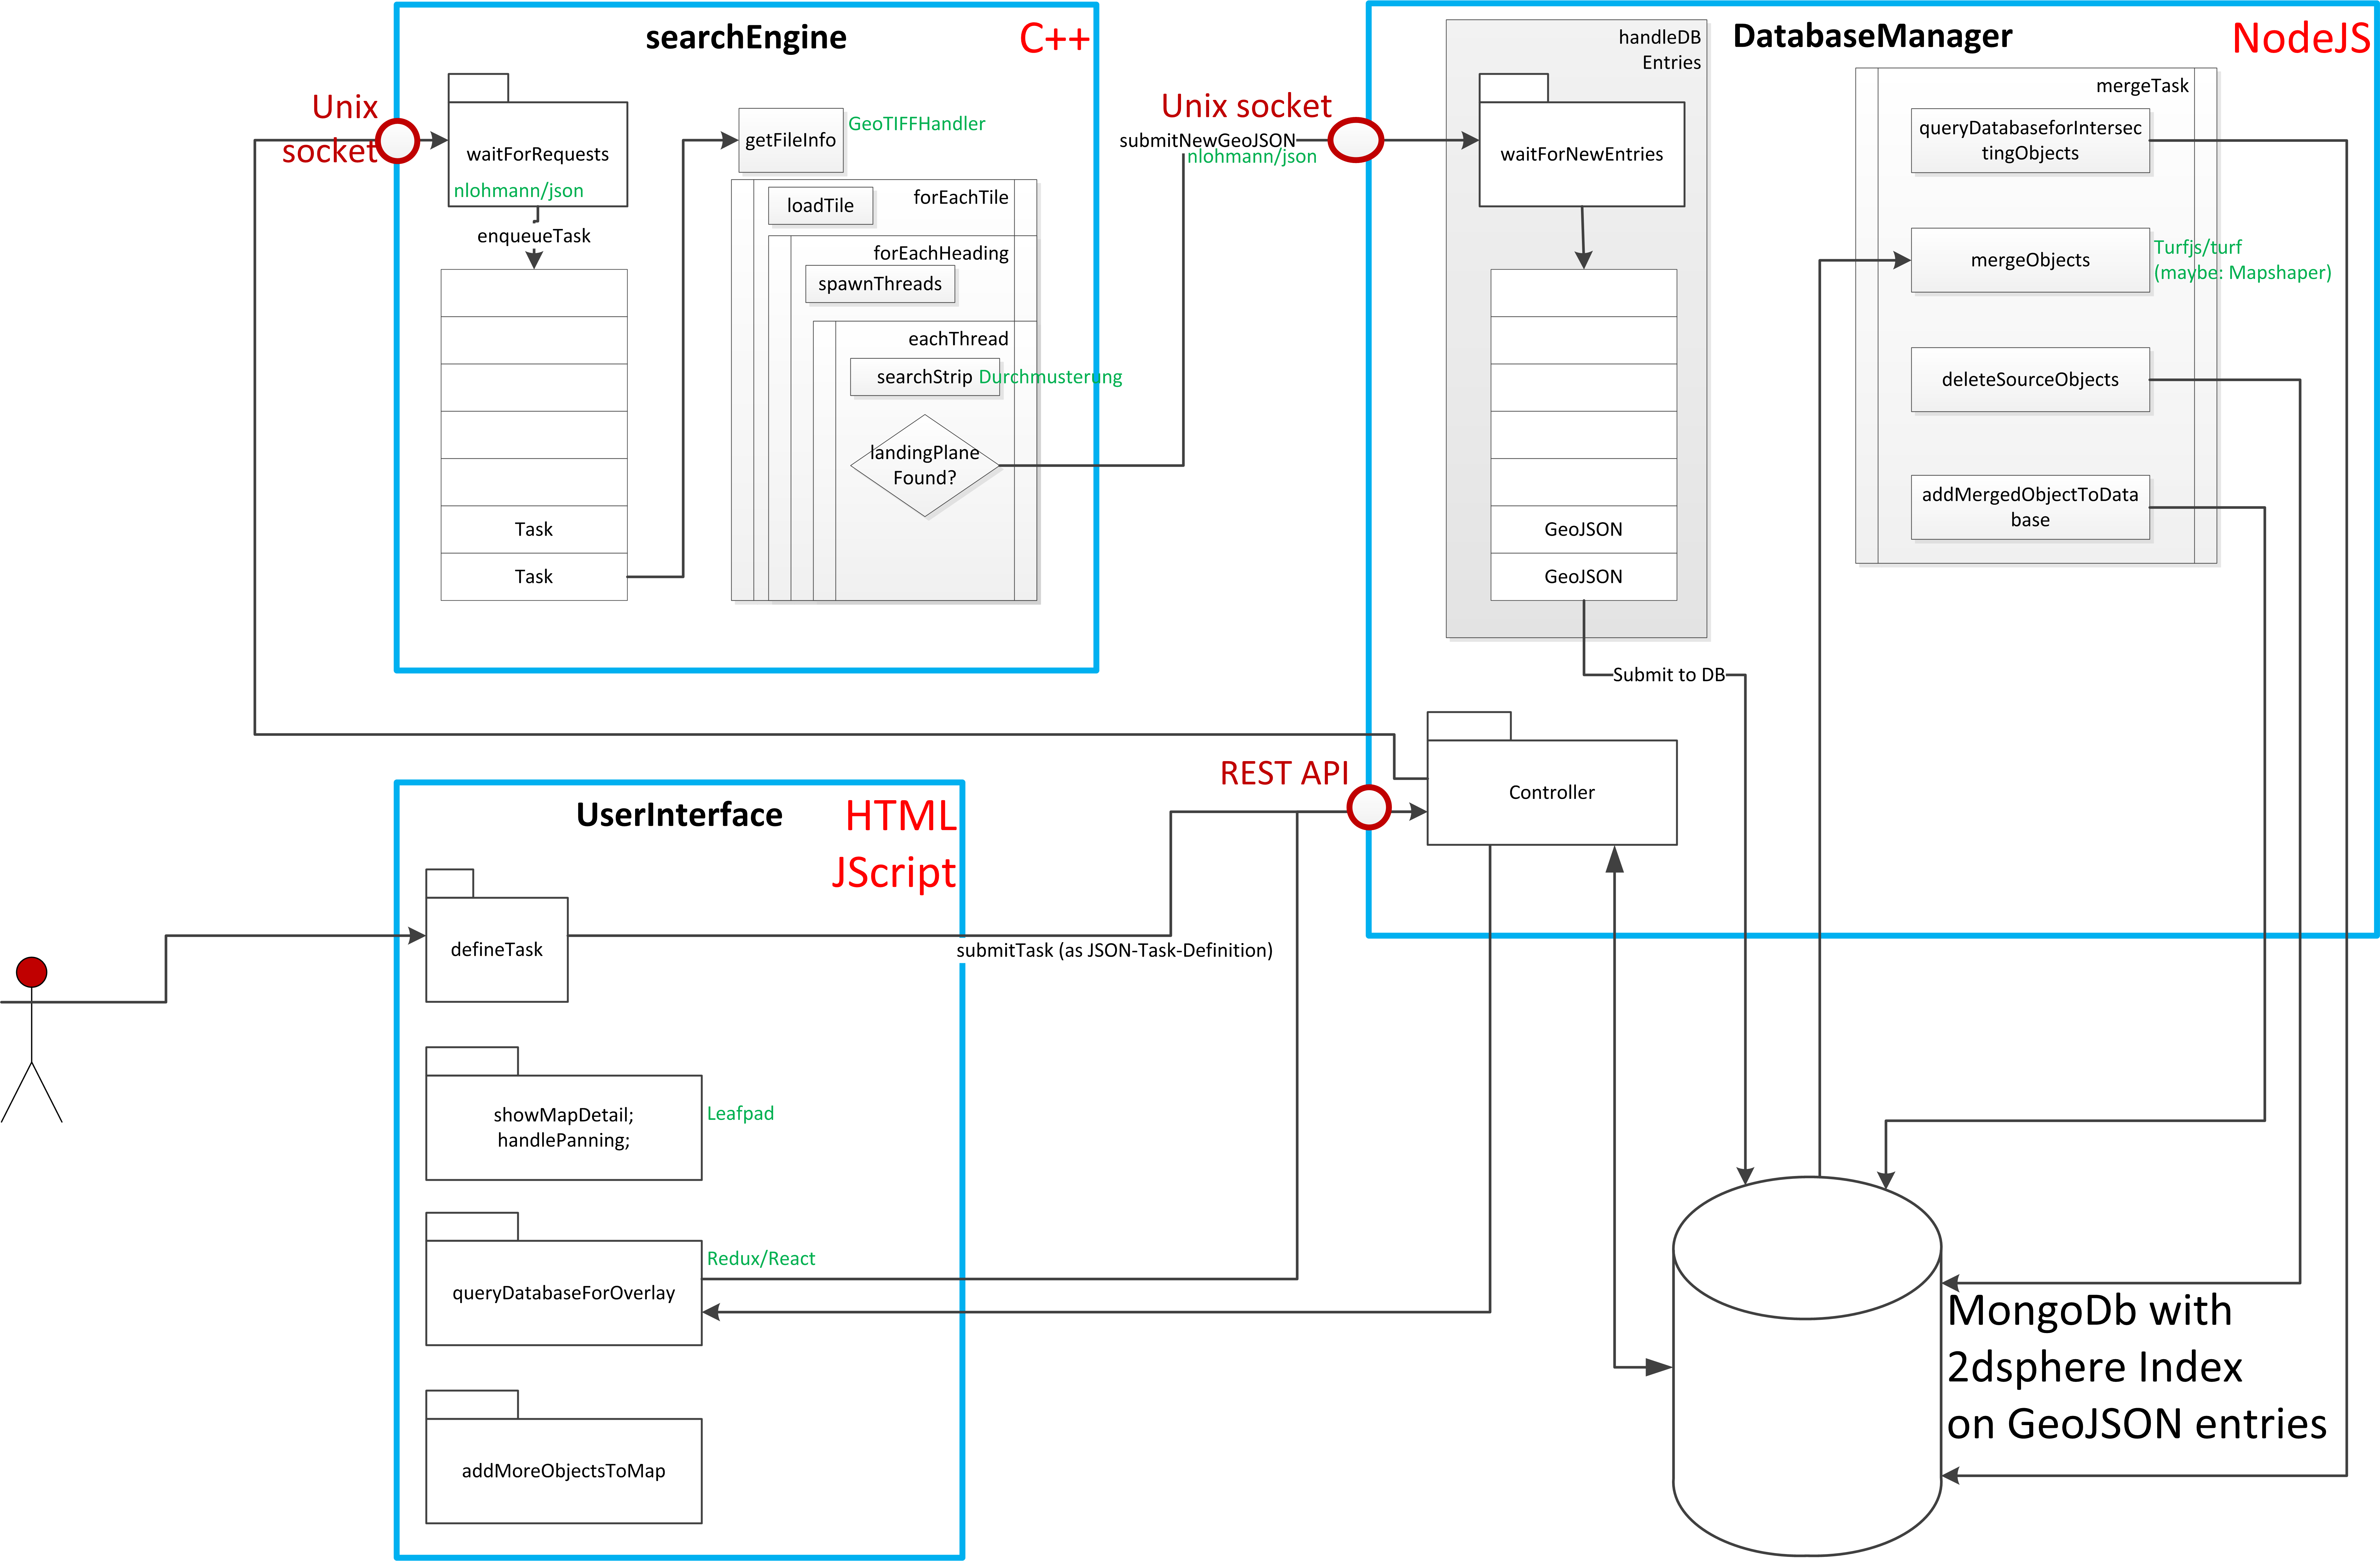
\includegraphics[width=\textwidth]{../Architektur/Architektur.png}
	\caption{Architekturüberblick} \label{architektur}
\end{figure}

Hier sind vier unabhängige Komponenten zu erkennen:
\begin{itemize}
	\item das UserInterface
	\item der DatabaseManager
	\item die SearchEngine
	\item die Datenbank
\end{itemize}

Abgebildet auf eine Model-View-Controller-Architektur (MVC) würde das User Interface der View entsprechen, der Database Manager dem Controller, die Datenbank dem Model. Die Search Engine ist der Geschäftslogik zuzuordnen und liegt kommuniziert ausschließlich über den Controller.
In der gezeigten Architektur fällt der mergeTask innerhalb des Database Managers etwas aus der Reihe. Dieser Task wurde erst relativ spät hinzugefügt um überlappende potentielle Landebahnen zu größeren Landefeldern zusammenzufassen. Dies ist ein Task, der grundsätzlich vollkommen unabhängig von allen anderen Aufgaben im Hintergrund ablaufen könnte und damit Teil der Geschäftslogik wäre. In der aktuellen Ausbaustufe wurde dieser Task jedoch aus Praktikabilitätsgründen zusammen mit dem Database Manager realisiert. Details dazu folgen in einem eigenen Abschnitt weiter unten.

In der Abbildung \ref{architektur} ist eingezeichnet in welcher Sprache/Programmiersystem die einzelnen Komponenten realisiert wurden. zusätzlich sind wichtige Komponenten und Bibliotheken in grün angegeben.

Die Kommunikation der Komponenten untereinander erfolgt über verschiedene Standard-Mechanismen:
\begin{itemize}
	\item lokale Unix Sockets zur Kommunikation des Database Managers mit der Search Engine.
	\item REST (Representational State Transfer) -API zur Kommunikation des User Interface mit dem Controller
	\item TCP/IP zur Kommunikation des Database Managers mit der Datenbank
\end{itemize}


\section{Grobkörnige Parallelität}
Aus der Abbildung ist ersichtlich, dass die vier Hauptkomponenten des Systems nur sehr lose gekoppelt sind. Die eingesetzten Kommunikationsprotokolle zwischen den Komponenten sind allesamt unabhängig von der konkreten physikalischen Verbindung. Die ausgetauschten Datenmengen zwischen den einzelnen Komponenten sind relativ klein. Daraus ergibt sich die Möglichkeit alle vier Komponenten auf unterschiedlichen Rechnern zu instantiieren und ablaufen zu lassen.

Damit ergibt sich schon eine gewisse, sehr grobkörnige Parallelität, welche bei Engpässen der Rechenleistung oder des Speichers für bestimmte Tasks ausgenutzt werden kann um die Gesamtperformance des Systems zu steigern. auch können für die einzelnen Aufgaben unterschiedliche, heterogene Maschinen eingesetzt werden. So stellt eine Datenbank andere Anforderungen an die Maschine als das Durchsuchen großer Datenmengen mit der Search Engine.

Ein weiterer Vorteil der konsequenten Trennung der View vom Rest der Software liegt darin, dass die Ergebnisse der Durchmusterung auch auf relativ schwachbrüstigen Geräten angezeigt werden können, welche lediglich über einen Javascript fähigen Browser und eine Netzwerkverbindung verfügen.

\section{Feingranulare Parallelität}

Während die grobkörnige Parallelität sich direkt aus der gewählten Architektur ergibt und quasi gratis kommt, so ergeben sich für die rechenintensive Aufgabe des Durchmusterns der Ausgangsdaten weitere Anforderungen, die über eine solche lose Kopplung hinausgehen.

Da inzwischen jeder halbwegs moderne Rechner über Mehrkernprozessoren und relativ viel gemeinsamen Speicher verfügt lag es nahe die rechenintensive Aufgabe der Datenanalyse explizit zu parallelisieren und dazu shared Memory Techniken zu nutzen. Genutzt wurden dafür im vorliegenden Lösungsvorschlag POSIX Threads, die mittels der \emph{pthreads}-Routinen eingebunden werden können.

Zusätzlich zu den Number-Crunching-threads, welche in der Bilbiothek "`Durchmusterung"' zur Performance-Steigerung eingesetzt werden, ist die gesamte Komponente searchEngine auf mehrere Threads aufgeteilt um eine reaktive Applikation zu realisieren. Details dazu werden im nächsten Kapitel erläutert.


\chapter{Komponente "`searchEngineWrapper"'}

Die Komponente "`searchEngineWrapper"' ist in C/C++ realisiert und dient dazu vom Controller Aufgaben entgegen zunehmen und auszuführen. Dazu gehört die Kommunikation mit der "`Außenwelt"' über UNIX-Sockets, die Verwaltung der Warteschlange mit Aufträgen, das Einlesen der Daten mit den dazugehörigen Koordinatentransformationen, die Aufteilung auf mehrere Kacheln falls nicht alle Daten in den Speicher passen und der Start der eigentlichen Durchmusterung.

Zur Kommunikation der Systembestandteile untereinander kommt das simple JSON-Format\footnote{siehe dazu \url{http://www.json.org/}} zum Einsatz. JSON bietet sich an, da für die Speicherung in der ausgewählten Datenbank sowieso JSON zum Einsatz kommt und dieses Datenformat von allen beteiligten Komponenten sehr gut unterstützt wird. In C++ lässt sich JSON sehr einfach über eine Open-Source Header-Only Bibliothek\footnote{siehe dazu: \url{https://github.com/nlohmann/json}} einbinden und dann wie native Objekte nutzen.

Die Komponente "`searchEngineWrapper"' startet zunächst zwei Threads: den \verb|queueDispatcher| und den \verb|ipcListener|. Der  \verb|ipcListener| lauscht permanent auf einem UNIX-Socket zur Interprozess-Kommunikation (IPC) und stellt von dort empfangene Aufträge in eine FIFO-Queue ein. Aus dieser FIFO-Queue entnimmt der \verb|queueDispatcher| nacheinander die Aufgaben und bringt sie zur Ausführung. Der Zugriff auf die Warteschlange wird mit Semaphoren und einer Conditional Variable geschützt, so dass bei leerer Warteschlange kein aktives Polling stattfinden muss, sondern der \verb|queueDispatcher| schlafen kann.

Der \verb|queueDispatcher| bringt die in der Warteschlange eingestellten Befehle nacheinander zur Ausführung. Er versteht dabei lediglich zwei Befehle: 
\begin{itemize}
	\item \verb|SCAN|: startet eine Durchmusterung eines bestimmten Kartenausschnitts nach potentiellen Notlandefeldern
	\item \verb|SAVE_2_M_FILE|: speichert die Höhenwerte der Eingabedaten eines bestimmten Kartenausschnitts in ein Matlab-kompatibles Dateiformat. Dies diente zu Beginn der Entwicklung dazu sich ein Bild der Daten zu machen und diese mit GNU Octave zu untersuchen.
\end{itemize}
Die Befehle kommen in Form von JSON-Objekten und enthalten alle notwendigen Parameter, die zur Ausführung benötigt werden.

Wenn ein \verb|SCAN| Task ausgeführt wird, so wird ein weiterer Thread aufgespannt, der sich zunächst um das einlesen der Rohdaten kümmert bevor er die als externe Bibliothek eingebundene Komponente "`Durchmusterung"' startet innerhalb derer das heavy lifting der Landebahnsuche stattfindet. Wie die Rohdaten verarbeitet werden wird gleich näher beschrieben.

Es wird immer nur ein \verb|SCAN|-Task auf einmal abgearbeitet, da benutzte Komponente "`Durchmusterung"' intern eine Parallelisierung durchführt und so die vorhandene Prozessorleistung so optimal ausnutzen kann. Eine Parallelisierung mehrere Tasks würde lediglich zu einer unnötigen Konkurrenz um Ressourcen führen ohne dass daraus mehr Performance erwachsen würde.

Durch die Aufteilung des "`searchEngineWrapper"' in mehrere parallele Threads (die sich meistens langweilen und auf externe Anweisungen warten) bleibt die Applikation auch dann reaktiv, wenn gerade eine Durchmusterung eines Bereichs durchgeführt wird, welche intern maximale Leistung von den zur Verfügung stehenden Kernen verlangt.

Bevor weitere Details der erstellten Software beschreiben werden, muss noch kurz auf die verwendeten Datenformate für Geodaten eingegangen werden:

\section{Datenformate und Verarbeitung}
Die Höhendaten werden, wie bei Geodaten üblich als sogenanntes GeoTIFF bereitgestellt. 

Die gefundenen potentiellen Landebahnen sind durch ein Rechteck charakterisiert, welches mitsamt bestimmten Parametern als GeoJSON in die Datenbank abgelegt wird.

\subsection{GeoTIFF}
Beim TIFF Format handelt es sich um ein Containerformat, das für einen rechteckigen Bereich aus Pixeln für jedes Pixel Informationen in den verschiedensten Datenformaten aufnehmen kann. Einen ersten Überblick gibt Wikipedia\footnote{siehe dazu \url{https://de.wikipedia.org/wiki/Tagged_Image_File_Format}} während die vollständige Spezifikation unter \url{https://www.loc.gov/preservation/digital/formats/fdd/fdd000022.shtml} abgerufen werden kann. Glücklicherweise ist es nicht notwendig diese Spezifikation selber zu implementieren. Es reicht aus einige Basiseigenschaften zu kennen und passende Bibliotheken zu benutzen.

Bei TIFF Dateien, wie sie im Geodaten-Bereich verwendet werden, handelt es sich um Ausschnitte der Erdkugel, welche auf eine rechteckige Ebene projiziert wurden. In dieser Ebene hat jedes Pixel eine feste Größe und jedem Pixel sind in verschiedenen Bändern diverse Daten zugeordnet. Im vorliegenden Fall handelt es sich um 20mx20m große Pixel denen jeweils ein FLOAT32-Wert mit Höheninformationen zugeordnet ist.
Da die zugrundeliegenden Daten nicht zwingend als Rechteck vorliegen (NRW ist \emph{kein} rechteckiges Land), wird ein bestimmter Zahlenwert als \verb|noDataValue| definiert welcher ungültige/nicht vorhandene Daten beschreibt.

Die Daten werden verlustfrei komprimiert gespeichert und können von speziellen Bibliotheken (meist basierend auf der Open-Source Bibliothek libTIFF\footnote{siehe dazu \url{http://www.libtiff.org/}}) eingelesen werden.

Neben den in der eigentlichen TIFF Datei kodierten Information gehört zu einem GeoTIFF-Datensatz noch ein sogenanntes World-File mit Informationen zur Lage und Projektion der Kugelkoordinaten in die Ebene. Mit Hilfe dieser Daten lässt sich jedem Pixel des TIFF eindeutig ein Punkt auf der Erdoberfläche zuordnen. Diese dateien werden üblicherweise zusammen mit dem GeoTIFF als sogenannte "`Sidecar-Files"' mitgeliefert, jedoch erlaubt das TIFF Format auch die direkte Einbettung dieser Informationen. Sie sind dann nicht mehr für den Menschen lesbar. 

\subsection{Speicherformat: GeoJSON}
Im Gegensatz zu dem rasterorientieren GeoTIFF Format ist für die Verwaltung der gefundenen potentiellen Landebahnen ein vektororientiertes Format deutlich besser geeignet. Wegen seiner Einfachheit, seiner weiten Verbreitung und der sehr guten Unterstützung durch die Datenbank fiel die Wahl auf das GeoJSON Format.

Ein GeoJSON Objekt ist ein einfaches JSON Objekt, welches die drei Properties \emph{type}, \emph{properties} und \emph{geometry} enthält. In der Property \emph{type} angegeben, ob es sich um nur eine Geometrie (\emph{type: Feature}) oder um einen mehrteiligen Satz von Geometrien (\emph{type: FeatureCollection}) handelt. In \emph{geometry} wird das Objekt selber spezifiziert. In unserem Fall handelt es sich um Polygone, deren Eckpunkte durch Koordinaten angegeben werden. In \emph{properties} schließlich können dem GeoJSON Objekt noch beliebige weitere Eigenschaften zugeordnet werden.

Die vollständige Spezifikation des Formats ist zu finden unter \url{https://geojson.org}. Ein sehr praktisches Tool um das Datenformat kennenzulernen und selber erstellte Datensätze auf Konformität zu testen findet sich unter \url{http://geojson.io}.

\section{GeoTIFFHandler}

Um den Umgang mit den GeoTIFF Daten zu kapseln wurde eine Klasse \emph{GeoTIFFHandler} entwickelt, welche nach Angabe eines Dateipfades ein GeoTIFF-File einliest und sich um die Verwaltung sämtlicher Metainformationen kümmert. Die Höhendaten werden der benutzenden anwendung direkt im Speicher zur Verfügung gestellt und können bequem zugegriffen werden, ohne dass sich um Speicherverwaltung oder Geodaten-Transformationen gekümmert werden muss. Für sehr große Datensätze, die nicht mehr komplett in den Speicher passen übernimmt die \emph{GeoTIFFHandler}-Klasse auch die Aufteilung in mehrere Kacheln und die dazu gehörende Speicherverwaltung.

Die einzelnen Funktionen werden weiter unten näher erläutert.

\subsection{Datenextraktion}
Der erste Schritt um mit einem Datensatz zu arbeiten ist die Extraktion der darin enthaltenen Daten. Wie oben schon erläutert wurde handelt es sich bei TIFF um ein sehr komplexes Format, das Dateien beliebiger Größe aufnehmen kann.

Da natürlich keine Routine zum Dekodieren diese Datenformats erstellt werden sollte wurden mehrere Bibliotheken gesichtet, die zum Einlesen der Daten in einem TIFF geeignet sind. Ein wichtiger Aspekt dabei war, dass die Bibliothek eine effiziente Einleseroutine für Teildaten eines großen Datensatzes bereitstellen soll. Da die Geodaten sehr groß werden können ist die Wahrscheinlichkeit gegeben, dass nicht der gesamte Datensatz auf einmal verarbeitet werden kann. Auch soll es möglich sein nur bestimmte Ausschnitte eines Datensatzes zu Durchmustern um dadurch auf eine kurze Durchmusterungszeit zu kommen.

Nach diesen Kriterien ausgewählt fiel die Wahl auf die Bibliothek "`LargeTIFFTools"'\footnote{siehe dazu: Deroulers et al., \href{http://www.diagnosticpathology.org/content/8/1/92}{Analyzing huge pathology images with open source software, Diagnostic Pathology 8:92 (2013)}.} und das darin enthaltene \texttt{tiffastcrop}. Diese Bibliothek lädt nicht das gesamte TIFF in den Speicher, bevor es einen Ausschnitt entnimmt, sondern lediglich die tatsächlich benötigten Teile. dies bringt nach Angaben des Bibliotheksautors dramatische Geschwindigkeitsvorteile gegenüber einer Reihe anderer gebräuchlicher Bibliotheken. (Diese Aussage konnte aufgrund fehlender "`großer"' Datensätze nicht überprüft werden. Das Laden der Bildausshnitte geht aber tatsächlich sehr schnell.) 

Mit Hilfe dieser Bibliothek ist die Klasse \texttt{GeoTIFFHandler} in der Lage jeden beliebigen rechteckigen Ausschnitt eines GeoTIFF-Datensatzes in den Speicher zu laden und dort die Höhendaten als \texttt{FLOAT32} zur Verfügung zu stellen.

Falls der angeforderte Ausschnitt zu groß ist um in den Speicher zu passen wird automatisch eine Kachelung vorgenommen.
In der folgenden Abbildung \ref{kachelung} ist das Prinzip dargestellt: Es wird festgestellt, wie groß ein rechteckiger Ausschnitt des angeforderten Ausschnitts maximal sein darf, damit er noch vollständig in den Speicher passt. Als Randbedingung gilt, dass angrenzende Kacheln um mindestens die minimale Landebahnlänge (z. B. 2000m) überlappen müssen. Dadurch ist sichergestellt, dass aufgrund von Kachelrändern keine potentiellen Bahnen übersehen werden. Das schlimmste, was dadruch passieren kann ist, dass eine potentielle Bahn in beiden Kacheln gefunden wird und dadurch doppelt in die Datenbank eingetragen wird.

\begin{figure}[ht]
\centering
	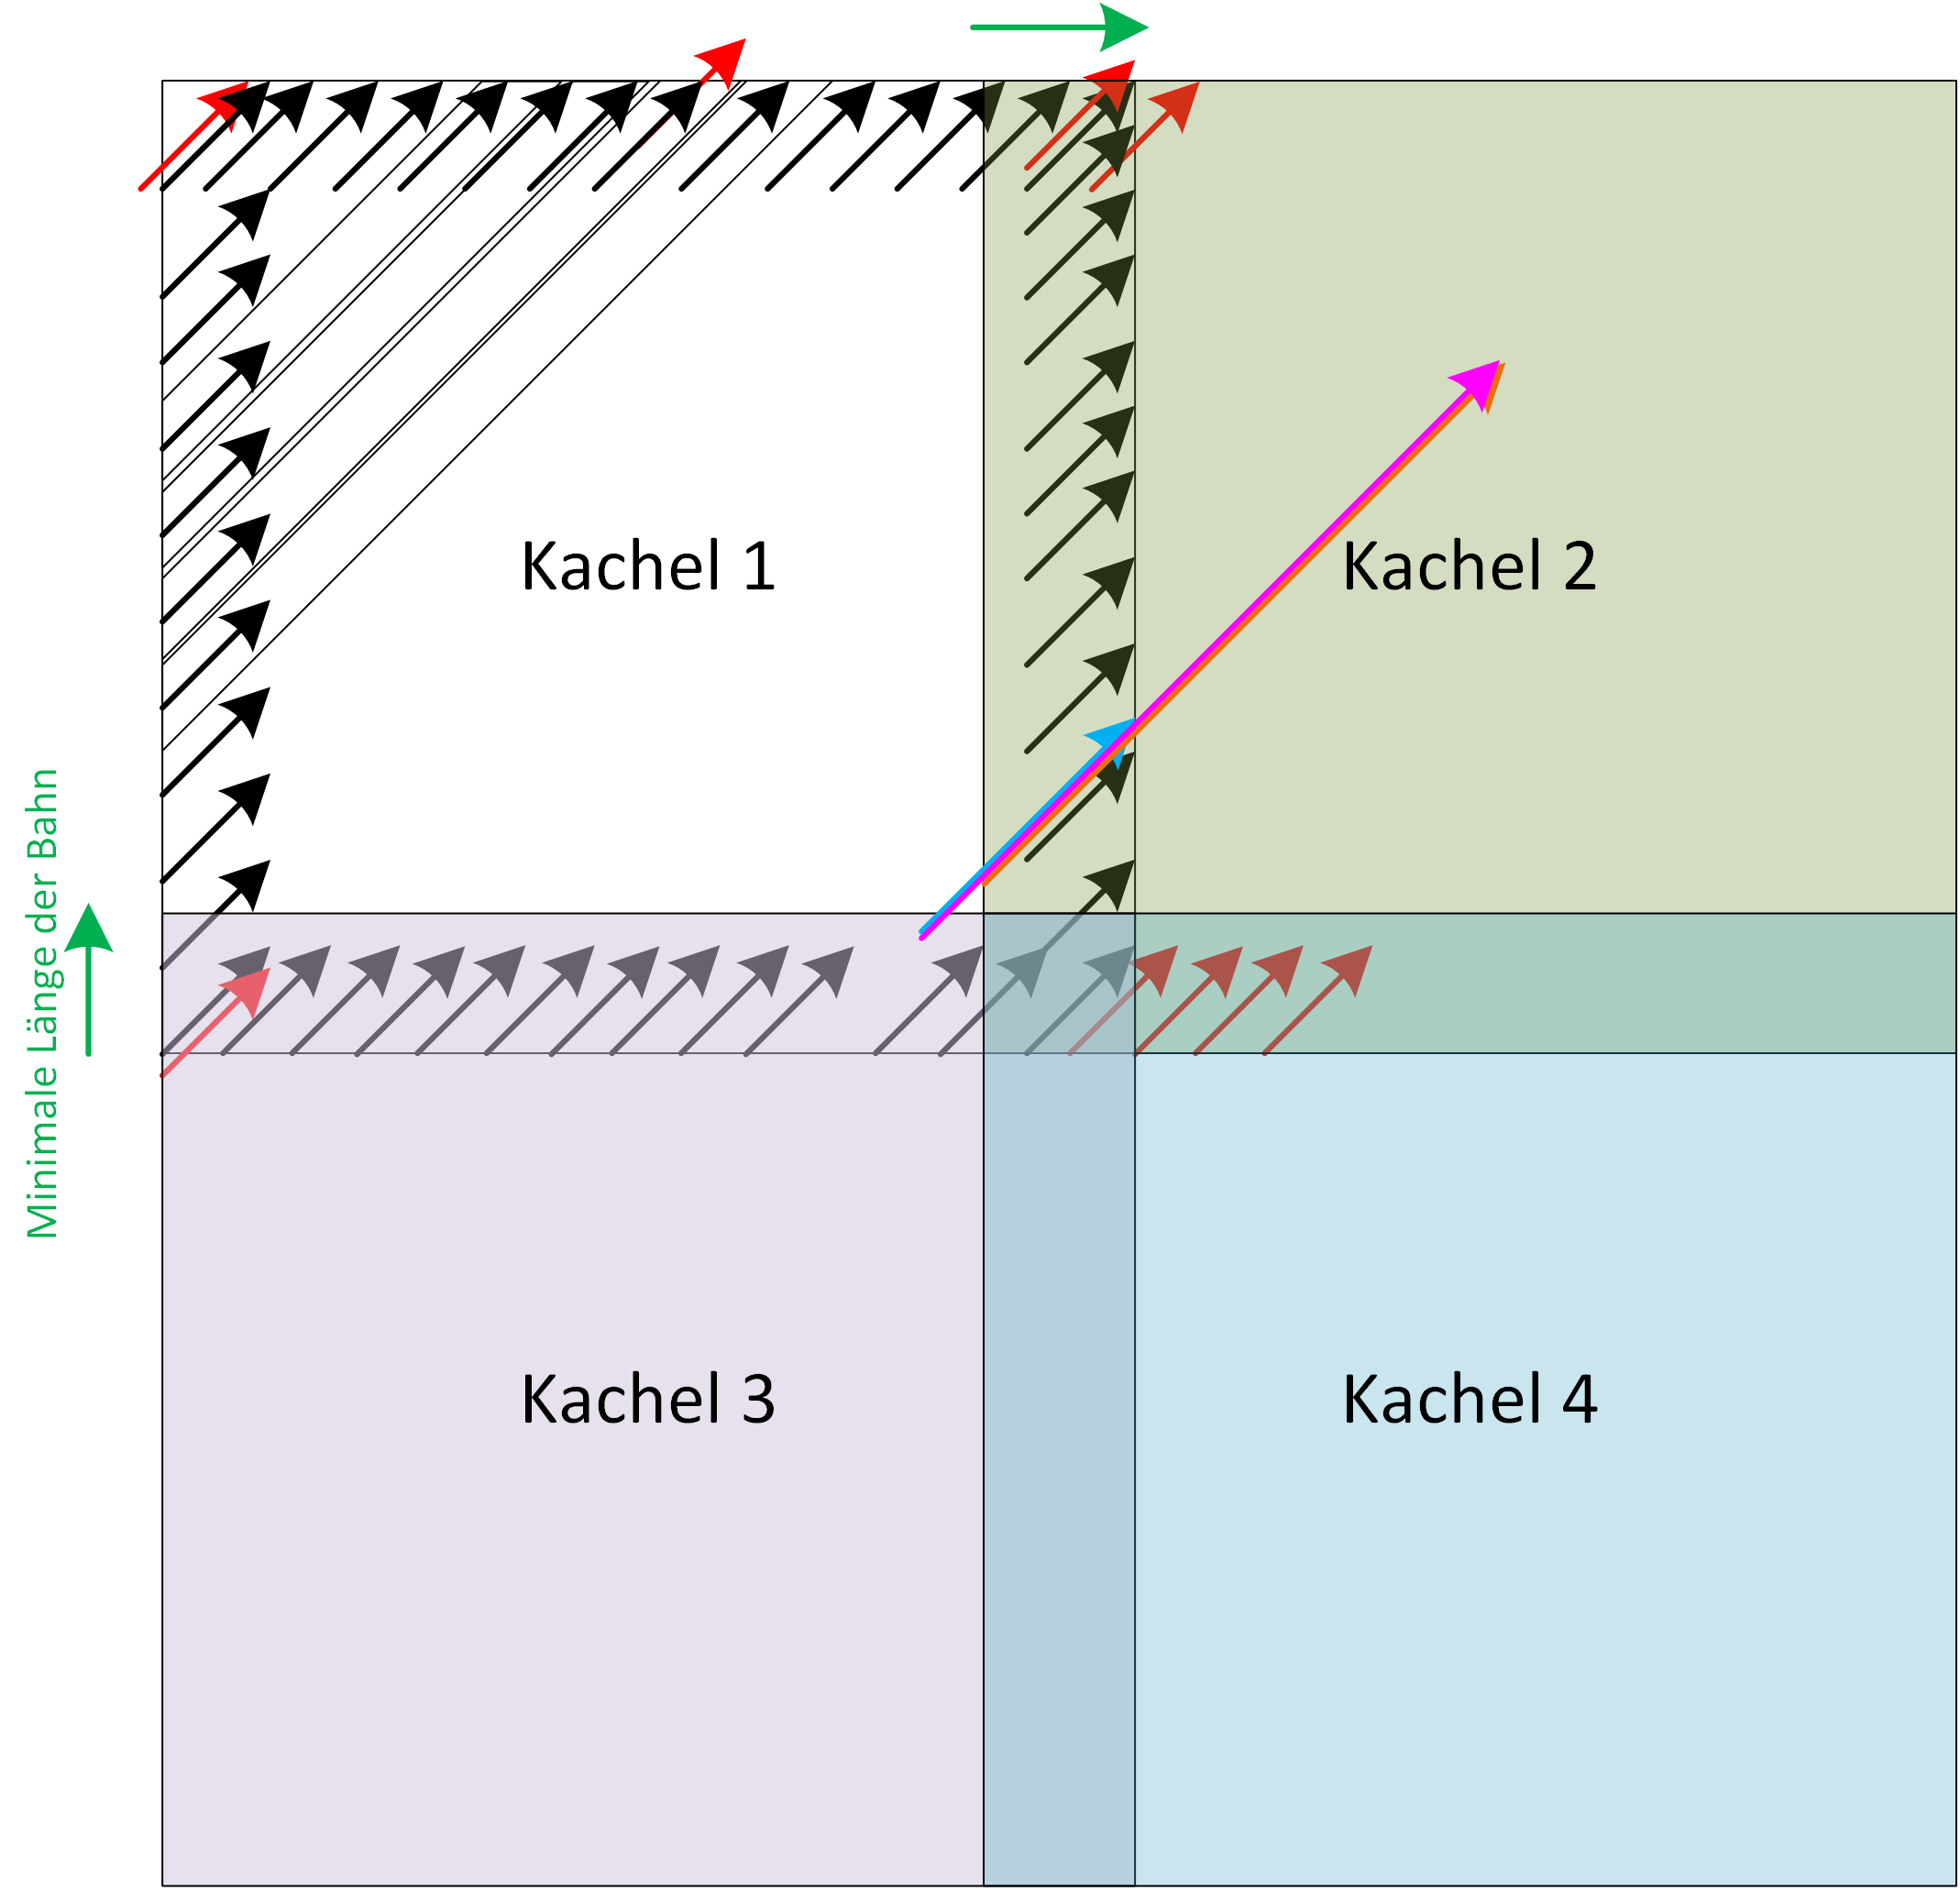
\includegraphics[width=0.5\textwidth]{../Vorgehensweise/drawings/UeberlappungKacheln.png}
	\caption{Prinzip der Kachelung bei Datensätzen, die nicht vollständig in den Speicher passen}
	\label{kachelung}
\end{figure}


In der aktuellen Implementierung ist eine künstliche Beschränkung auf die Hälfte des noch zur Verfügung stehenden RAMs eingestellt.\footnote{Der noch maximal zur Verfügung stehende Speicher lässt sich ermitteln über \texttt{size\_t maxUsableRAM = sysconf(\_SC\_AVPHYS\_PAGES) * sysconf(\_SC\_PAGESIZE);}}. Dies könnte in künftigen Versionen leicht geändert werden, war aber mit den vorhandenen Datensätzen nicht notwendig.

\subsection{Koordinatensysteme}

Eine große Herausforderung bei der Verarbeitung von Geodaten stellen die verwendeten Projektionen und Koordinatensysteme dar. Da es nicht möglich ist eine Kugeloberfläche (genauer eine Elipsoidoberfläche) gleichzeitig Längen- und Winkeltreu auf eine Ebene zu projizieren, existiert eine Vielzahl verschiedener Projektionssysteme, welche immer einen gewissen Kompromiss aus den gewählten Anforderungen darstellen. So listet allein die \href{http://geotiff.maptools.org/proj_list/}{GeoTIFF Projections Transform List} über 40 verschiedene, offensichtlich gängige Projektionen für GeoTIFF Datensätze auf.

Glücklicherweise gibt es eine sehr umfangreiche und relativ gut dokumentierte open source Bibliothek, welche die Umrechnung der verschiedenen Projektionen und Koordinatensysteme abstrahiert und zur Verfügung stellt. Diese \href{http://www.gdal.org/}{GDAL - Geospatial Data Abstraction Library} kommt auch in diesem Projekt zum Einsatz und ermöglicht es auf relativ einfache Art und Weise die Daten aus dem GeoTIFF zu extrahieren und mit Koordinaten im WGS84-Koordinatensystem\footnote{siehe hierzu als Einstieg: \href{https://de.wikipedia.org/wiki/World_Geodetic_System_1984}{https://de.wikipedia.org/wiki/World\_Geodetic\_System\_1984}} in Einklang zu bringen. Das WGS84 System ist das aktuell in der Luftfahrt verwendete Koordinatensystem und wird auch in Navigationssystemen und insbesondere in Kartendiensten im Internet verwendet. Koordinaten im WGS84-System werden über die bekannten zwei Werte von geographischer Länge (Longitude) und geographischer Breite (Latitude) angegeben. Die Büro von Prof. Schiffmann an der Fernuniversität Hagen hat in diesem System z. B. die Koordinaten \href{http://bl.ocks.org/d/94faa16e1c8cb9d9226902f9fb0cc36c}{Lat: 51.37632449291616N, Long:7.493609189987183E}

Mit Hilfe der erwähnten Bibliothek werden innerhalb der Klasse \texttt{GeoTIFFHandler} Funktionen bereitgestellt, die von WGS84-Koordinaten auf Pixel im Speicher und umgekehrt umrechnen können. Damit kann die Durchmusterung auf einem reinen Pixel basierten Koordinatensystem erfolgen, während Zuordnung von Geokoordinaten vollständig aus dem Durchmusterungsprozess heraus abstrahiert ist. Es muss dem GeoTIFF-Handler lediglich am Anfang mitgeteilt werden, welcher rechteckige Ausschnitt (in Geokoordinaten) aus dem Datensatz eingelesen werden soll. die Durchmusterung findet dann auf einem rechteckigen Pixelbereich statt. Gefundenen Bahnen werden über Ihren Anfangs- und Endpunkt in Pixel-Koordinaten und Ihre Breite charakterisiert und vom \texttt{GeoTIFFHandler} auf Koordinaten in WGS84 abgebildet.

\paragraph{Schwäche der vorliegenden Implementierung:} Leider hat sich zum Ende der Bearbeitungszeit herausgestellt, dass bei einem Datensatz in der Größe von NRW die zuvor getroffene Annahme falsch ist, dass das GeoTIFF-Pixel-Rechteck an jeder Stelle in Nord-Süd- bzw. Ost-West-Richtung ausgerichtet ist. In der vorliegenden Implementierung wird implizit davon ausgegangen, dass der rechte Nachbar eines jeden Pixels genau in östlicher (also 90\degree) Richtung liegt und der untere Nachbar in südlicher (also 180\degree) Richtung. Das ist aber aufgrund der schon erwähnten Probleme mit der Projektion eines Elipsoiden auf eine Ebene nicht korrekt und so ergeben sich über die gesamte Fläche Abweichungen von wenigen Grad, wenn diese Annahme bei der Durchmusterung auf Pixel-ebene aufrecht erhalten wird. Da es sich bei der vorliegenden Implementierung bisher noch eher um einen Proof-of-Concept handelt wurden diese Abweichungen von der geforderten Richtung toleriert. Im Ausblick wird ein möglicher Lösungsansatz angesprochen um dieses Problem zu lösen.


\subsection{Das \emph{GeoTIFFHandler}-Objekt}

Die Suchmaschine hält sich während der Programmlaufzeit ein \texttt{GeoTIFFHandler}-Objekt, welches die gesamte Interaktion mit der GeoTIFF-Datei inklusive der gerade beschriebenen Transformationen übernimmt.

Dieses Objekt stellt der Suchmaschine folgende Daten zur Verfügung:

\begin{lstlisting}[language=c]
struct datasetInfo {
	pixelPair extent = {0,0};	
		//the extent of the current dataset
	rectSize pixelSize = {0,0}; 	
		//dimension of a single pixel in [meter]
	float noDataValue = 0;	//marker for "no data" in the dataset;
		//the marker value for invalid/non existant pixels
};	
\end{lstlisting}

Dies sind die für die Durchmusterung relevanten globalen Daten über den Datensatz. Die Koordinaten der Eckpunkte können über die Funktion \verb|geoCoord pixel2Geo(const pixelCoordFloat source);| abgefragt werden, falls das nötig ist. Wesentlich ist vor allem die Angabe des "`ungültig Werts"' innerhalb der Pixel im Speicher.

Sobald der Benutzer eine Auswahl getroffen hat, welchen Bereich der Welt er nach Notlandefeldern durchmustern möchte kann über den Aufruf der Funktion 
\begin{lstlisting}[language=c]
resultType getTilingInfo(const geoCoord topLeft, const geoCoord bottomRight,
		const float overlap, const size_t maxSize, 
		tilingCharacteristics *tilingResult);
\end{lstlisting}

das \texttt{GeoTIFFHandler}-Objekt angewiesen werden das einlesen der Daten in den Speicher vorzubereiten und Informationen darüber bereitzustellen, ob die Daten eventuell in mehreren Kacheln verarbeitet werden müssen. Dazu wird eine spezielle Datenstruktur gefüllt:
\begin{lstlisting}[language=c]
struct tilingCharacteristics {
	int overallXSize = 0, overallYSize = 0;	
		//the extent of the currently requested cutout of the dataset
	pixelCoord topLeftPix = {0,0};	
		//top left pixel coordinate of the requested area
	pixelCoord bottomRightPix = {0,0};	
		//bottom right pixel coordinate of the requested area
	int maxTileSizeXPix = 0, maxTileSizeYPix = 0;
	int overlapXPix =0, overlapYPix =0;
	int tilesInX = 0, tilesInY = 0;	
		//the amount of tiles in X- and Y-direction
	float overlap = 0;	
		//the overlap of the tiles in [meter]
	size_t maxTileMemsize = 0;	
		//the maximum amount of bytes a tile needs in memory
};
\end{lstlisting}

Diese Angaben sind ausreichend um die Durchmusterung auf Pixelebene zu beginnen. Das \texttt{GeoTIFFHandler}-Objekt kann angewiesen werden nacheinander die einzelnen Kacheln (oder auch nur die eine Kachel) in den Speicher zu laden, so dass sie durchsucht werden können. Die gesamte Speicherverwaltung wird duch den \texttt{GeoTIFFHandler} übernommen, weswegen vor dem Laden der nächsten Kachel auch die aktuell verwendete Kachel explizit wieder freigegeben werden muss.

Zusätzlich werden noch einige Datenstrukturen und Hilfsfunktionen zur Verfügung gestellt, die (hoffentlich einigermaßen ) selbsterklärend sind.
Die wesentlichen zur Verfügung gestellten Funktionen sind:
\begin{lstlisting}[language=c]
	resultType getDatasetInfo(datasetInfo *info);
	resultType getPixelExtent(rectSize *pixelSize);
	resultType getTilingInfo(const geoCoord topLeft, 
			const geoCoord bottomRight, const float overlap, 
			const size_t maxSize, 
			tilingCharacteristics *tilingResult);
	resultType getTile(const int xTile, const int yTile, tileData *tile);
	resultType releaseTile(const int xTile, const int yTile);

	geoCoord pixel2Geo(const pixelCoordFloat source);
	geoCoord pixel2Geo(const int xTile, const int yTile, 
			const pixelCoordFloat source);
	pixelCoord geo2Pixel(const geoCoord source);
	pixelCoord geo2Pixel(const int xTile, const int yTile, 
			const geoCoord source);

	/**
	 * returns a valid geoJSON Object with empty properties
	 * These have to be overwritten later on.
	 * see https://gis.stackexchange.com/questions/144084/
	 		using-gdal-c-to-calculate-distance-in-meters
	 * see https://geographiclib.sourceforge.io/1.40/
	 		C/inverse_8c_source.html
	 */
	json getGeoJsonPolygon(const pixelCoordFloat start, 
			const pixelCoordFloat end, const float width);
	json getGeoJsonPolygon(const pixelCoordFloat start, const float length, 
			const float heading, const float width);
	json getGeoJsonPolygon(const pixelCoordFloat pix0, 
			const pixelCoordFloat pix1, const pixelCoordFloat pix2, 
			const pixelCoordFloat pix3);
\end{lstlisting}

\chapter{Komponente "'Durchmusterung"'}
\section{Durchmusterung der Geotiff Daten und Auffinden der Landebahnen}
Die Durchmusterung der Geodaten wurden in einer eigenen statischen Library gekapselt ($plane\_library.a$). Innerhalb dieser Library finden sich alle Algorithmen, die zum Auffinden der Landebahnen benötigt werden. Für den Aufrufer ist die Implementation komplett gekapselt. Alle funktionalen Requirements werden von dieser Library übernommen.


\section{Interface der Library}

Die Parameter des Interfaces sind im Listing \ref{interface} beschrieben.

\begin{lstlisting}[caption=Interface Beschreibung, label=interface]
int search_for_planes(const tileData *actualTile, 
GeoTiffHandler *myGeoTiffHandler, 
float heading, float minLength, float width, int commSocket,
const json *taskDescription, float noDataValue , rectSize pixelSize );
\end{lstlisting}

Die einzelnen Aufrufparameter und deren funktionale Eigenschaft sind in Tabelle~\ref{beschreibungparameter} aufgezeigt.

\begin{table}[htb]
\centering
\begin{tabular}{|p{4.5cm}|p{10cm}|}
\hline 
\bf{Parameter} & \bf{Funktion} \\ 
\hline 
*actualTile & Zeiger auf das Geo-Kartenobjekt mit den individuellen Höhendaten \\ 
\hline 
*myGeoTiffHandler & Zeiger auf eine Instanz eines GeoTiffHandler Objekts, 
welches diverse Funktionen zur Umrechnung, Konvertierung etc. im GeoTiff Format unterstützt \\ 
\hline 
heading & Durchmusterungswinkel für die Landebahnen $0^\circ =>$ Nord-Süd Achse \\ 
\hline 
minLength & minimale geforderte Länge der Landebahn in [m] \\ 
\hline 
width & Breite der geforderten Landebahn in [m] \\ 
\hline 
commSocket & Socket für das abspeichern gefundener Landebahnen in der Mongo DB\\ 
\hline 
*taskDescription & Taskbeschreibung, um die gefundene Bahn korrekt in der Mongo DB abzulegen \\ 
\hline 
noDataValue & Zahlenwert für undefinierte Kartenpunkte \\ 
\hline 
pixelSize & Auflösung der Rasterpunkte in [m]\\
\hline 

\end{tabular} 
\caption{Beschreibung der Aufrufparameter Funktionalität}\label{beschreibungparameter}
\end{table}

\section{logischer Ablauf innerhalb der Landebahn Erkennung}

Der logische Ablauf ist schematisch im Nassi-Shneiderman-Diagramm~\ref{nasshnlogisch} dargestellt.

\clearpage
\begin{figure}
\begin{struktogramm}(100,200)\label{nasshnlogisch}
  \assign{Initialisisierung $tile\_worker$ Objekt}
  \assign{Berechne winkel-, steigungs- und holprigkeitsabhängige Parameter}
\forallin{Für alle Startpunkte einer Landebahn in gegebener Richtung (Thread Pool)}
\assign{wähle den nächsten Punkt}
\ifthenelse[15]{1}{1}
{kurzreichweitige Steigung zum Vorgänger OK?}{\sTrue}{\sFalse}
\ifthenelse[17]{1}{6}
{checke Holprigkeit in Querrichtung}{\sTrue}{\sFalse}
\change
\ifthenelse[25]{1}{1}
{ist die aktuelle Landebahn länger als die Mindestlänge}{\sTrue}{\sFalse}
\assign{Suche die beste Landebahn mit Mindestlänge}
\assign{Speichere beide Landebahnen in der Mongo DB}
\assign{starte eine neue Landbahn mit aktuellem Punkt}
\change
\assign{starte eine neue Landbahn mit aktuellem Punkt}
\ifend
\ifend
\change
\ifthenelse[30]{1}{1}
{ist die aktuelle Landebahn länger als die Mindestlänge}{\sTrue}{\sFalse}
\assign{Suche die beste Landebahn mit Mindestlänge}
\assign{Speichere beide Landebahnen in der Mongo DB}
\assign{starte eine neue Landbahn mit aktuellem Punkt}
\change
\assign{starte eine neue Landbahn mit aktuellem Punkt}
\ifend
\assign{starte eine neue Landbahn mit aktuellem Punkt}
\ifend
\forallinend
\end{struktogramm}
\caption{Durchmusterungsalgorithmus in Pseudo-Code}
\end{figure}
\clearpage
\section{Initialisierung}

Die Initialisierung erzeugt zunächst ein $tile\_worker$ Objekt und initialisiert die Instanzvariablen mit den bei der Objekterzeugung angegebenen Durchmusterungscharakteriska wie maximal erlaubte Steigung, Varianz und minimale Landebahnlänge.
Mit dem Aufruf von $check\_steigungen()$ werden dann die optimalen Schrittvektoren und die Startkoordinaten des Durchmusterungsvorgangs bestimmt.

Die optimalen Durchmusterungsvektoren sind winkelabhängig. Die Idee hierbei ist, dass in Abhängigkeit der Auflösung diese Vektoren so initialisiert werden, dass alle möglichen Landebahnen gefunden werden. Dies führt dazu, dass bestimmte Winkel beim Durchmustern dichtere Landebahnen abtasten können. Somit wird sichergestellt, dass jede Landebahn mindestens einmal untersucht wird.
Zusätzlich dazu werden dann orthogonale Vektoren aus den Schrittvektoren abgeleitet, die zum Durchmustern in orthogonaler Richtung (Landebahnbreite) benutzt werden.

Anhand der gegebenen Kartenauflösung und Schrittvektoren kann dann bestimmt werden, wie viele aufeinander folgende Punkte mindestens benötigt werden, damit die Landebahn die Mindestlängenvoraussetzung erfüllt.
Entsprechendes gilt natürlich auch für die Breite der Bahn.

Anschließend werden dann die Startpunkte der Durchmusterung bestimmt.
Diese sind abhängig vom Durchmusterungswinkel. 
Für Winkel, die ein vielfaches von 90 betragen, wird einfach eine Seite des Quadranten abgeschritten. Wird eine Bahn z.B. in $y$-Richtung abgetastet, wird der Abzissenwert inkrementiert / dekrementiert und erneut in $y$-Richtung abgeschritten, bis der Rand der Kachel erreicht wird. Eine schematische Abbildung findet sich in Abbildung~\ref{scanortho}.

Bei Winkeln, die nicht einem Vielfachen von 90 entsprechen, werden sukzessiv sowohl Abszisse als auch Ordinate abgeschritten und das Terrain in Diagonaler Richtung durchmustert. 
Eine schematische Abbildung hierzu findet sich in Abbildung~\ref{scandiagonal}. Hier wird zunächst die Abszisse bis zum Ursprung abgeschritten, bevor der Ordinatenwert inkrementiert wird.

\begin{figure}\label{scandiagonal}
\centering
\begin{tikzpicture}
\draw[help lines, color=gray!30, dashed] (0,0) grid (4.9,4.9);
\draw[->,ultra thick] (0,5)--(5,5) node[right]{$x$};
\draw[->,ultra thick] (0,5)--(0,0) node[left]{$y$};

\draw[-,ultra thick] (5,5)--(5,0) node[left]{};
\draw[-,ultra thick] (0,0)--(5,0) node[right]{};

\draw[->,ultra thick,dashed,red] (4,5)--(5,4) node[left]{$1$};
\draw[->,ultra thick,dashed,red] (3,5)--(5,3) node[left]{$2$};
\draw[->,ultra thick,dashed,red] (0,5)--(5,0) node[right]{$3$};

\draw[->,ultra thick,dashed,red] (0,3)--(3,0) node[below]{$4$};

\draw[->,ultra thick,dashed,red] (0,1)--(1,0) node[below]{$5$};

\draw[-,ultra thick,dashed,blue] (5,5.5)--(-0.5,5.5) node[left]{};
\draw[->,ultra thick,dashed,blue] (-0.5,5.5)--(-0.5,0) node[left]{};
\end{tikzpicture}
\caption{Verschiebung des Startpunkts der Landebahndurchmusterung in diagonaler Richtung. Hier NNO nach SSW. Der Startpunkt der einzelnen Bahnen folgt dem blauen Pfeil.}
\end{figure}


\begin{figure}\label{scanortho}
\centering
\begin{tikzpicture}
\draw[help lines, color=gray!30, dashed] (0,0) grid (4.9,4.9);
\draw[->,ultra thick] (0,5)--(5,5) node[right]{$x$};
\draw[->,ultra thick] (0,5)--(0,0) node[left]{$y$};

\draw[-,ultra thick] (5,5)--(5,0) node[left]{};
\draw[-,ultra thick] (0,0)--(5,0) node[right]{};

\draw[->,ultra thick,dashed,red] (0,5)--(0,0) node[below]{$1$};
\draw[->,ultra thick,dashed,red] (1,5)--(1,0) node[below]{$2$};
\draw[->,ultra thick,dashed,red] (3,5)--(3,0) node[below]{$3$};
\draw[->,ultra thick,dashed,red] (5,5)--(5,0) node[below]{$4$};


\draw[->,ultra thick,dashed,blue] (-0,5.5)--(5,5.5) node[left]{};
\end{tikzpicture}
\caption{Verschiebung des Startpunkts der Landebahndurchmusterung in diagonaler Richtung. Hier N nach S. Der Startpunkt der einzelnen Bahnen folgt dem blauen Pfeil.}
\end{figure}
\section{Parallelverarbeitung mittels p\_threads zum Finden der Landebahnen}

Die Parallelverarbeitung arbeitet nach einem Task-Workermodell, welches mit einem Semaphor gesteuert wird. Jeder Startpunkt, der auf einem Kartenrand liegt, ist hier als ein Task anzusehen. Das Semaphor dient dazu, die gleichzeitige Anzahl der Threads zu steuern und zu kontrollieren. Dies dient zum einen Untersuchungszwecken, um festzustellen, die der Speedup bei Variation der Threads ist. Weiterhin würde eine zu hohe Zahl an an Threads die ausführende Maschine in extreme Ressourcenknappheit bringen können.

Das Workerobjekt kontrolliert mit einem mutex die Herausgabe von Startwerten. In einem kritischen Bereich wird durch Inkrementierung des Startpunktes ein neuer Startpunkt generiert, der an einen Worker als Form eines abzuarbeitenden Task herausgegeben wird. Dieser kritische Bereich, der dafür sorgt, dass jeder Startpunkt auch nur wirklich einmal herausgeben wird, stellt somit auch das Bottleneck der Parallelverarbeitung dar. So lange die Anzahl der Punkte pro Bahn und die Berechnungszeit, die ein Thread benötigt, um die Bahn in der vorgegebenen Richtung abzuscannen und die zur Bahn gehörigen Parameter wie Varianz etc. zu berechnen größer ist als die Zeit, die vergeht, bis der Thread wieder in der Warteschlange zum Erhalt eines neuen Startwert aufläuft, sollte dieses Bottleneck gering sein.

Zudem ist zu beachten, dass natürlich nicht alle Landebahnen gleich lang sind. So lange der Startpunkt in der Nähe einer Kartenecke ist und die Durchmusterungsrichtung nur wenige Punkte bis zum Kartenrand umfasst, wird die Durchmusterung schnell vorbei sein und ein neuer Startwert benötigt werden. Dies wird in Abbildung~\ref{scandiagonal} deutlich. Mit der potentiellen Landebahn 3 hat der Thread die meisten Punkte abzuarbeiten während die Bahnen 1 und 5 relativ schnell abgearbeitet seien werden. 

\section{Detaillierte Beschreibung des Suchalgorithmus}

Ausgehend vom jeweiligen Startpunkt wird mittels $p\_thread\_create$ ein neuer Thread erzeugt und die Funktion $void *thread\_data::check\_single\_plane(void *x\_void\_ptr)$ als Startroutine mitgegeben. Innerhalb dieses erzeugten Threads existiert eine while Schleife, die solange true returniert, wie noch nicht alle Startpunkte an Threads ausgeben wurden.

Innerhalb einiger verschachtelten Bedingungen wird überprüft, ob der betrachtete Geopunkt tatsächlich Höheninformationen hat und ob die Steigung zu seinem unmittelbaren Vorgänger innerhalb des erlaubten Bereiches liegt.

Trifft dies zu, so ist noch die Steigung benachbarter Punkte in orthogonaler Richtung zu betrachten. Sind all diese Kriterien erfüllt, wird der betrachtete Geopunkt in eine Liste an gültigen Punkten aufgenommen. Diese Prozedur wird so lange wiederholt, bis ein Kriterium nicht mehr erfüllt ist oder der Kartenrand erreicht ist.

Ist eines dieser Abbruchkriterien erfüllt, wird überprüft, ob das Ensemble aneinanderhängender Punkte die Mindestlänge der geforderten Landebahn erfüllt.

Dann wird eine Subroutine $find\_best\_planes()$ aufgerufen, welche innerhalb der gefunden Liste an zusammenhängenden Punkten zwei Landebahnen ermittelt. Zum einen wird die längste Bahn, die das Steigungskriterium erfüllt ermittelt und des weiteren die Landebahn, die die geringste Varianz aufweist und trotzdem noch die geforderte Mindestlänge erreicht. 
Beide Bahnen werden dann in einer Mongo DB abgelegt.

\section{Klassen und Objekte}

In der $plane\_library.a$ werden mehrere Klassenimplementationen verwendet, um objektorientiert zu einer vereinfachten Problemlösung zu gelangen.

Die zentrale Klasse ist dabei die $tile\_worker$-Klasse. In ihr werden wichtige Membervariablen zu den parametrisierten Rahmenbedingungen verwaltet und das Threading mittels p\_thread abgehandelt. Die Klasse $landing\_plane$ beschreibt ein Hilfsobjekt, in dem gefundene Landebahnobjekte via Startpunkten, Steigung und Varianz beschrieben wird.
Das Threading selbst hat eine sehr schlanke $thread\_data$-Klasse, welche in einer \glqq friend\grqq -Beziehung zum $tile\_worker$ steht und sich ausschließlich mit der Parallelausführung beschäftigt.

Der $tile\_manager$ ist eine Klasse, die ausschließlich zu Debug- und Entwicklungszwecken zum Bau eines Standalone Binaries benötigt wird.
Für den produktiven Einsatz ist sie obsolet.


\section{Verwendete Datenstrukturen}

Die wichtigsten Datenstrukturen, die während der Durchmusterung benötigt werden, sind das übergebene Kachelobjekt, ein Objekt zur Verwaltung der aktuell gefundenen zusammenhängenden Punkte, sowie der $tile\_worker$, der die Threads kontrolliert und Durchmusterungsparameter kapselt. 

\subsection{Einfluss der Datenstrukturen auf die Performanz}

Die Container-Klasse des $tile\_worker$ hat in seiner endgültigen Form keine komplexeren Datenstrukturen mehr. Sie beinhaltet lediglich Membervariablen einfacher Datentypen wie $double$ und $int$.

Innerhalb der Thread-Klasse findet sich eine lokale Variable $coordlist$, welche vom Typ $vector< pair<int,int> >$ ist.
Hier werden temporär aneinanderhängende Ketten von Landebahnpunktkoordinaten vorgehalten. Die gespeicherten Punkte sind dabei lediglich Referenzen auf das statische Kartenobjekt. Ohne dieses wären die Informationen bedeutungslos.

Der Vorteil des vector templates in C++ ist der optimierte random access, welcher in der Komplexizitätsklasse O(1) zu finden ist und die Verwaltung sehr komfortabel mittels Member-Funktionen vorgegeben ist.

Das Kachelobjekt selbst stellt die Höheninformationen eines 2-dimensionalen Kartenausschnitts in einem linearen Array dar. Der Durchmusterungsalgorithmus benötigt allerdings einen Mappingmechanisumus eines 2-dimensionalen Punktes auf das eindimensionales Array.

Dies wird von der Funktion $access\_single\_element(int\ x, int\ y)$ bereitgestellt. Anhand der Information, wie viele Datenpunkte der Kartenausschnitt in $x$-Richtung beinhaltet, wird das Mapping auf das eindimensionale Array dargestellt. Im Falle einer Bereichsüberschreitung, wird $numeric\_limits<float>::min()$ zurückgegeben.
Auch dieser Zugriff ist der Komplexitätsklasse O(1) zuzuordnen und unabhängig von Datengröße.

\begin{lstlisting}
float tile_worker::access_single_element(int x, int y)
{
  if (tile->width.x*y+x < tile->width.x*tile->width.y)
    return(tile->buf[tile->width.x*y+x]);
  else
   return numeric_limits<float>::min();

}
\end{lstlisting}

Dies führt dazu, dass der Speicherbedarf ausschließlich von der Anzahl der Datenpunkte in den Rohdaten abhängig ist. Für die Speicherallokierung werden insbesondere bei den C++ Templates vordefinierte default-Allokatoren genutzt, die man natürlich mit eigens definierten überladen könnte. Dafür gibt es bislang aber keinerlei Notwendigkeit.
 


\section{Bestimmung des Speedups in Abhängigkeit des Parallelisierunggrades}

Um den Speedup zu bestimmen, wurde analysiert, wie sich die Laufzeit mit zunehmender Anzahl an Threads verändert. So lange die Bearbeitung einer einzelnen Bahn viel länger dauert als die in der kritischen Sektion benötigte Zeit, um einen neuen Startpunkt zu bestimmen, sollten die Threads nicht blockiert sein.

Bei Winkeln, die ein vielfaches von $90$ betragen, sind alle Landebahnen gleich lang --- also sind gleich viele Punkte zu analysieren (siehe Abbildung~\ref{scanortho}).

Bei Bahnen, die diagonal verlaufen, sind die ersten Bahnen kurz, nehmen dann in ihrer Länge zu, bis als Startpunkt die nächstliegende Ecke erreicht ist, und nimmt dann in ihrer Länge wieder ab (siehe Abbildung~\ref{scandiagonal}). 
Weiterhin ist zu beachten, dass je nach Topologie der Bahn unterschiedlich viele (im Grenzfall gar keine) geeignete Flächen gefunden werden, die dann fein granular weiter untersucht werden müssen (längste Bahn und die mit der kleinsten Varianz). So ist schwer vorhersagbar, wie lange die Einzellaufzeit eines Threads ist.
Für die zur Verfügung gestellten Kartendaten von Nordrhein-Westfalen sind die Laufzeiten in Abhängigkeit von Winkel und Threadanzahl in Tabelle~\ref{laufzeiten} dargestellt.

\subsection{Erläuterung des Messverfahren}

Die Messung wurde in einer virtualisierten Umgebung durchgeführt. Als Host-System diente ein Windows 7 64 bit System, welches hardwaretechnisch auf einem Intel i7-4770K , 3.5 Ghz, 16 GB RAM System lokalisiert ist. Die Virtualisierung wurde mit Virtualbox mit einem Linux Guest System (Centos Linux 7.0, 6 GB RAM) durchgeführt. 
Die Anzahl der virtuellen CPUs wurde von 1-8 variiert.
Pro vorgegebener Parametrisierung wurden 4 unabhängige identische Messungen gemacht. In Tabelle~\ref{laufzeiten} angegeben ist der Mittelwert mit Standardabweichung dieser Läufe.
 

\subsection{Messergebnisse}
\begin{figure} 
\begin{tabular}{|c|c|c|c|c|c|}
\hline 
Richtung & Bahnen & Threads & v CPUs & Zeitbedarf [ms] & Standardabweichung [ms] \\ 
\hline 
N$\rightarrow$S (0$^\circ$) & 734 & 1 & 1 & 11409 & 510 \\ 
\hline 
N$\rightarrow$S (0$^\circ$) & 734 & 2 & 1 & 11049& 216 \\ 
\hline 
N$\rightarrow$S (0$^\circ$) & 734 & 4 & 1 & 11586 & 220 \\ 
\hline 
N$\rightarrow$S (0$^\circ$) & 734 & 8 & 1 & 11230 & 240 \\ 
\hline 
N$\rightarrow$S (0$^\circ$) & 734 & 64 & 1 & 10886 & 621 \\ 
\hline 
W$\rightarrow$O (90$^\circ$) & 1606 & 1 & 1 & 10442 & 239 \\ 
\hline 
W$\rightarrow$O (90$^\circ$) & 1606 & 64 & 1 & 10094 & 284 \\ 
\hline 
NNO$\rightarrow$SSW (45$^\circ$) & 704 & 1 & 1 & 18147 & 327 \\ 
\hline 
NNO$\rightarrow$SSW (45$^\circ$) & 704 & 64 & 1 & 18423 & 701 \\ 
\hline 
N$\rightarrow$S (0$^\circ$) & 734 & 1 & 2 & 8488 & 46 \\ 
\hline 
N$\rightarrow$S (0$^\circ$) & 734 & 2 & 2 & 5397 & 178 \\ 
\hline 
N$\rightarrow$S (0$^\circ$) & 734 & 4 & 2 & 5545 & 161 \\ 
\hline 
W$\rightarrow$O (90$^\circ$) & 1606 & 1 & 2 & 8668 & 453 \\ 
\hline 
W$\rightarrow$O (90$^\circ$) & 1606 & 2 & 2 & 5778 & 292 \\ 
\hline 
NNO$\rightarrow$SSW (45$^\circ$) & 704 & 1 & 2 & 15208 & 216 \\ 
\hline 
NNO$\rightarrow$SSW (45$^\circ$) & 704 & 64 & 2 & 8976 & 327 \\ 
\hline
N$\rightarrow$S (0$^\circ$) & 734 & 1 & 4 & 8823 & 83 \\ 
\hline 
N$\rightarrow$S (0$^\circ$) & 734 & 2 & 4 & 4642 & 77 \\ 
\hline 
N$\rightarrow$S (0$^\circ$) & 734 & 4 & 4 & 2973 & 17 \\ 
\hline 
N$\rightarrow$S (0$^\circ$) & 734 & 8 & 4 & 3571 & 432 \\ 
\hline 
W$\rightarrow$O (90$^\circ$) & 1606 & 8 & 4 & 3335 & 72 \\ 
\hline 
NNO$\rightarrow$SSW (45$^\circ$) & 704 & 8 & 4 & 5406 & 442 \\ 
\hline
N$\rightarrow$S (0$^\circ$) & 734 & 16 & 8 & 2733 & 56 \\ 
\hline 
\end{tabular}
\caption{Laufzeiten verschiedener Durchmusterungen in Abhängigkeit der Threads und virtuellen CPUs}\label{laufzeiten}
\end{figure} 

\subsection{Diskussion der Messergebnisse}

Als Landebahneigenschaften wurden eine Länge von 4000~m, eine Holprigkeit in Längs- und Querrichtung von 3~\%, sowie eine maximale Steigung von 10~\% gefordert. Dieses Parameterset wurde so gewählt, dass nicht zu viele Landebahnen in die Datenbank geschrieben werden müssen, da dies auch einen signifikanten CPU Anteil benötigt. Weiterhin ist das Rendering im Browser bei sehr vielen bahnen CPU intensiv. Daher erschien das oben gewählte Parameterset als schlüssig.
Auffällig ist, dass selbst im Singlethreadbetrieb bei der Erhöhung der CPUs ein Speedup entsteht. Dies ist dem Umstand geschuldet, dass auf derselben VM noch der Browser und die Datenbankengine gehostet sind.
Trotzdem wird das Parameterset 1 CPU, 1 Thread als Referenz für den Speedup betrachtet.

\begin{figure}
\begin{tabular}{|c|c|}
 \hline 
 Anzahl CPU & Speedup \\ 
 \hline 
 1 & 1 \\ 
 \hline 
 2 & 2,11 \\ 
 \hline 
 4 & 3,84 \\ 
 \hline 
  8 & 4,2 \\ 
 \hline 
 \end{tabular}  
 \caption{Speedup am Beispiel der Messergebnisse in Nord / Südausrichtung.}
\end{figure}

\begin{figure}
\begin{tabular}{|c|c|}
 \hline 
 Anzahl CPU & Speedup \\ 
 \hline 
 1 & 1 \\ 
 \hline 
 2 & 1,8 \\ 
 \hline 
 4 & 3,13 \\ 
 \hline 
 \end{tabular}  
 \caption{Speedup am Beispiel der Messergebnisse in Ost / Westausrichtung.}
\end{figure}

\begin{figure}
\begin{tabular}{|c|c|}
 \hline 
 Anzahl CPU & Speedup \\ 
 \hline 
 1 & 1 \\ 
 \hline 
 2 & 2,02 \\ 
 \hline 
 4 & 3,35 \\ 
 \hline 
 \end{tabular}  
 \caption{Speedup am Beispiel der Messergebnisse in Nordnordwest / Südsüdostausrichtung.}
\end{figure}

Weiterhin zeigt sich, dass eine weitere Erhöhung der Threadanzahl über die tatsächlich verfügbaren CPUs ab einem gewissen Punkt schädlich ist.
Im Falle von 8 CPUs sind die Ergebnisse unter Umständen nicht aussagekräftig, da die Virtualisierungssoftware eine ungültige Konfiguration anzeigte. Zudem braucht auch das Host Betriebssystem Ressourcen, die natürlich nicht der VM und der Software zur Verfügung stehen.

\begin{tikzpicture} 
\begin{axis}[ 
  xlabel=Anzahl CPU, ylabel=Speedup] 
  \addplot[color=red,mark=x] coordinates { 
  (1,1) 
  (2,2.11) 
  (4,3.84) 
  (8,4.2)   
  }; 
    \addplot[color=blue,mark=x] coordinates { 
  (1,1) 
  (2,1.8) 
  (4,3.13)    
  }; 
    \addplot[color=green,mark=x] coordinates { 
  (1,1) 
  (2,2.02) 
  (4,3.35)    
  }; 
  
  \end{axis} 
  
  \end{tikzpicture}
  
Eine weiterführende Analyse war aufgrund mangelnder Hardwareressourcen nicht möglich.


\section{Analyse mittels Profiler}

Mittels gproof wurde analysiert, welche Programmteile beim Auffinden der Landebahn die meiste Rechenzeit benötigen. Hierdurch kann kontrolliert werden, ob die vom Scheduler zur Verfügung gestellten Zeitscheiben auch effektiv innerhalb des Threadings genutzt werden können. 

Bei der Analyse zeigt sich, dass die Funktion, die die meiste Zeit in Anspruch nimmt, die Zugriffsfunktion auf die Geopunkte ist. Hier findet ein Random Memory access statt (2-Dimensionalität wird auf ein eindimensionales Array abgebildet).
Eine weitere zeitintensive Funktion stellt die Berechnung der Varianz sowie das Auffinden der längsten und der varianzminimalen Landebahn dar.

Diese Ergebnisse sind intuitiv zu erwarten.
Da beide Funktionen innerhalb des Threading aufgerufen werden, ist aus laufzeittechnischer Sicht eine optimale Lösung gefunden. 

\section{Einfluss von Compiler Direktiven (speziell Optimizer)}

Bevor Codeausführung mittels Parallelverarbeitung zur Beschleunigung gebracht werden soll, lohnt es sich meist, durch geeignete Compilerdirektiven die serielle Codeausführung zu beschleunigen.

Der Code wurde mit einem gcc Version 4.8.5 devtoolset version 4 compiliert. Die Standardübersetzung ist dabei ohne eingeschalteten Optimizer. 
Durch die Benutzung des -O3 Optimizer Direktivs ist eine Codebeschleunigung von 1300 \% (11 sec vs. 147 sec) beobachtet worden. 
Eine Übersicht über die verwendeten Optimierungsschritte sind unter https://gcc.gnu.org/onlinedocs/gcc/Optimize-Options.html einzusehen.

\chapter{Komponente "`databaseManager"'}


\section{Datenbankauswahl}
\section{Express-Server App}
\section{Postprocessing - Merge}

\chapter{Komponente "'landingClient"'}
\section{Überblick}
\section{Features und Bedienung}
  
\chapter{Ausblick und weitere Ideen}

Im Rahmen der Untersuchungen mit der im Praktikum erarbeiteten Softwarelösung sind einige verblüffende und interessante Artefakte sichtbar geworden.
Unabhängig von dem Winkel der Landebahn zeigte sich, dass der südöstliche Teil von NRW keine geeigneten Landebahnen bietet. Dies ist der Tatsache geschuldet, dass dort Gebirgszüge wie das Süderbergland und das Sauerland zu finden sind.
Entlang der niederländischen Grenze und an der Grenze zu Niedersachsen ist das Gebiet flacher.
Weiterhin ist überraschend, dass die ca 100 Mio Datenpunkte in so kurzer Zeit und mit so wenig Speicherbedarf bearbeitet werden können. Selbst auf einer kleinen virtuellen Maschine lief die Durchmusterung sehr zügig.
Weiterhin war überraschend, dass die Programmübersetzung mit optimiertem Code eine extreme Beschleunigung brachte.
Diese konnte durch das Threading noch weiter gesteigert werden.
Allerdings zeigt sich auch, dass vermutlich schon bei recht kleiner Parallelität (4-fach parallel) der Speed-up nicht mehr linear mit Anzahl der Prozessoren korreliert.
Die Berechnung der Varianz der Landebahn bzw. das Auffinden der optimalen Landebahnen aus einer Fläche benötigt in sich schon relativ viele Rechenoperationen. Hier könnte nochmals eine feingranulare eine Parallelisierung vorgenommen werden.
Es könnten weitere Parameter eingeführt werden, um noch mehr Randbedingungen an die Qualität einer Landebahn zu stellen. Dieses benötigt aber sicherlich noch mehr domänenpezifischen Input.
Interessant wäre es, Datensets mit mehr Datenpunkten und die Laufzeit bei diesen Randbedingungen zu untersuchen. Insbesondere, wenn die Fläche in eine größere Anzahl von Subkacheln gesplittet wird.
 
\section{Richtungskorrektur des GeoTIFF}
\section{Push für Webclient}
\section{Merge als nachgeschalteter Prozess aus dem Speicher}
\section{Kollisionsabfrage mit Objekten aus OSM}
\section{Parallele Bearbeitung mehrerer Kacheln per MPI}
Besonders bei größeren Datensätzen wäre es interessant, die Laufzeiteigenschaften der Software zu untersuchen. Bei sehr großen Datensätze wäre ein embedding in eine MPI Lösung vielleicht interessant, das die Daten innerhalb eines Clusters verteilt. Pro Knoten könnte dann mit Threading eine feingranulare Parallelisierung durchgeführt werden.
\end{document}
